\documentclass[conference]{IEEEtran}
% QONTOS Research Paper Series — Shared LaTeX Preamble
% Use with: % QONTOS Research Paper Series — Shared LaTeX Preamble
% Use with: % QONTOS Research Paper Series — Shared LaTeX Preamble
% Use with: \input{qontos-preamble}

\usepackage{cite}
\usepackage{amsmath,amssymb,amsfonts}
\usepackage{graphicx}
\usepackage{textcomp}
\usepackage{xcolor}
\usepackage{hyperref}
\usepackage{booktabs}
\usepackage{multirow}
\usepackage{array}
\usepackage{tabularx}
\usepackage{float}
\usepackage{listings}
\usepackage{url}
\usepackage{enumitem}

% Listing style
\lstset{
  basicstyle=\ttfamily\footnotesize,
  breaklines=true,
  frame=single,
  backgroundcolor=\color{gray!10},
}

% Custom column type
\newcolumntype{L}[1]{>{\raggedright\arraybackslash}p{#1}}

% QONTOS colors
\definecolor{qontosnavy}{HTML}{0A1628}
\definecolor{qontosblue}{HTML}{1E88E5}
\definecolor{qontosteal}{HTML}{00BCD4}

% Hyperref setup
\hypersetup{
  colorlinks=true,
  linkcolor=qontosblue,
  citecolor=qontosblue,
  urlcolor=qontosteal,
}

% Author block
\newcommand{\qontosauthor}{%
\IEEEauthorblockN{QONTOS Research Wing}
\IEEEauthorblockA{
Zhyra Quantum Research Institute (ZQRI)\\
Advanced Quantum Systems Division\\
Abu Dhabi, UAE\\
\texttt{research@zhyra.xyz}}
}


\usepackage{cite}
\usepackage{amsmath,amssymb,amsfonts}
\usepackage{graphicx}
\usepackage{textcomp}
\usepackage{xcolor}
\usepackage{hyperref}
\usepackage{booktabs}
\usepackage{multirow}
\usepackage{array}
\usepackage{tabularx}
\usepackage{float}
\usepackage{listings}
\usepackage{url}
\usepackage{enumitem}

% Listing style
\lstset{
  basicstyle=\ttfamily\footnotesize,
  breaklines=true,
  frame=single,
  backgroundcolor=\color{gray!10},
}

% Custom column type
\newcolumntype{L}[1]{>{\raggedright\arraybackslash}p{#1}}

% QONTOS colors
\definecolor{qontosnavy}{HTML}{0A1628}
\definecolor{qontosblue}{HTML}{1E88E5}
\definecolor{qontosteal}{HTML}{00BCD4}

% Hyperref setup
\hypersetup{
  colorlinks=true,
  linkcolor=qontosblue,
  citecolor=qontosblue,
  urlcolor=qontosteal,
}

% Author block
\newcommand{\qontosauthor}{%
\IEEEauthorblockN{QONTOS Research Wing}
\IEEEauthorblockA{
Zhyra Quantum Research Institute (ZQRI)\\
Advanced Quantum Systems Division\\
Abu Dhabi, UAE\\
\texttt{research@zhyra.xyz}}
}


\usepackage{cite}
\usepackage{amsmath,amssymb,amsfonts}
\usepackage{graphicx}
\usepackage{textcomp}
\usepackage{xcolor}
\usepackage{hyperref}
\usepackage{booktabs}
\usepackage{multirow}
\usepackage{array}
\usepackage{tabularx}
\usepackage{float}
\usepackage{listings}
\usepackage{url}
\usepackage{enumitem}

% Listing style
\lstset{
  basicstyle=\ttfamily\footnotesize,
  breaklines=true,
  frame=single,
  backgroundcolor=\color{gray!10},
}

% Custom column type
\newcolumntype{L}[1]{>{\raggedright\arraybackslash}p{#1}}

% QONTOS colors
\definecolor{qontosnavy}{HTML}{0A1628}
\definecolor{qontosblue}{HTML}{1E88E5}
\definecolor{qontosteal}{HTML}{00BCD4}

% Hyperref setup
\hypersetup{
  colorlinks=true,
  linkcolor=qontosblue,
  citecolor=qontosblue,
  urlcolor=qontosteal,
}

% Author block
\newcommand{\qontosauthor}{%
\IEEEauthorblockN{QONTOS Research Wing}
\IEEEauthorblockA{
Zhyra Quantum Research Institute (ZQRI)\\
Advanced Quantum Systems Division\\
Abu Dhabi, UAE\\
\texttt{research@zhyra.xyz}}
}


\begin{document}

\title{Distributed Quantum Software Stack: From Implemented Orchestration Platform to Modular Operating Layer}

\author{\qontosauthor}

\maketitle

\begin{abstract}
Quantum computing systems that span multiple interconnected processor modules require a software stack qualitatively different from the single-device compilers and runtimes available today. This paper describes the QONTOS software stack in two distinct registers: (i)~the \textbf{currently implemented} orchestration platform, which operates today on classical simulators and provides circuit ingestion, partitioning, scheduling, execution dispatch, result aggregation, and full observability; and (ii)~the \textbf{target extension} of that platform toward a modular operating layer designed for future multi-module quantum hardware with cross-module entanglement, real-time calibration feedback, and fault-tolerant workload management.

\textbf{[Claim: IMPLEMENTED]} The QONTOS platform exists today as a working software system. All orchestration, partitioning, scheduling, aggregation, and proof-of-execution capabilities described in Sections~2--4 run on simulator backends and are available in the public repository. \textbf{[Claim: TARGET]} The modular runtime extensions described in Sections~5--8---including hardware-aware placement, cross-module timing, digital-twin validation, and fault-tolerant control---represent architectural targets informed by current distributed quantum computing research (Monroe et al.\ 2014; Cuomo et al.\ 2020). These extensions do not yet execute on physical quantum hardware.

We frame this separation explicitly because honest delineation between present capability and future ambition is essential for credible quantum systems research.
\end{abstract}

\section{Introduction}

\subsection{The Software Gap in Modular Quantum Computing}

The quantum computing community has made substantial progress on single-device software toolchains. Frameworks such as Qiskit~\cite{Qiskit2023}, PennyLane~\cite{Bergholm2022}, and t$|$ket$\rangle$~\cite{Sivarajah2020} provide circuit construction, optimization, and transpilation for monolithic processors. Comparative surveys confirm the breadth of these gate-level platforms~\cite{LaRose2019}. However, as quantum systems scale beyond single-chip qubit limits, the software challenge shifts from circuit optimization to distributed orchestration: partitioning circuits across modules, scheduling inter-module entanglement operations, managing heterogeneous calibration states, and aggregating results with provenance guarantees.

\textbf{[Claim: CONTEXT]} No production-grade distributed quantum operating system exists today at any organization. The field is in an early-architecture phase. QONTOS contributes to this space by building an orchestration platform now---on simulators---that is designed from the ground up for the distributed case.

\subsection{Design Philosophy}

The QONTOS software stack follows three guiding principles:

\begin{enumerate}
\item \textbf{Software-first development.} Build the orchestration, partitioning, and runtime layers before hardware is available, using simulator backends as execution targets.
\item \textbf{Separation of implemented and target capability.} Every component in the stack is labeled by its current maturity. This prevents overstatement.
\item \textbf{Explicit connection to the repository.} All claims about implemented capability correspond to modules in the public QONTOS codebase (\url{https://github.com/qontos}). Where code does not yet exist, the paper says so.
\end{enumerate}

\subsection{Scope}

This paper covers the software and runtime layers. It connects to Paper~01 (Scaled Architecture), Paper~03 (Error Correction), Paper~05 (AI Decoding), and Paper~09 (Benchmarking).

\section{Current Implemented Platform}

\begin{figure}[t]
\centering
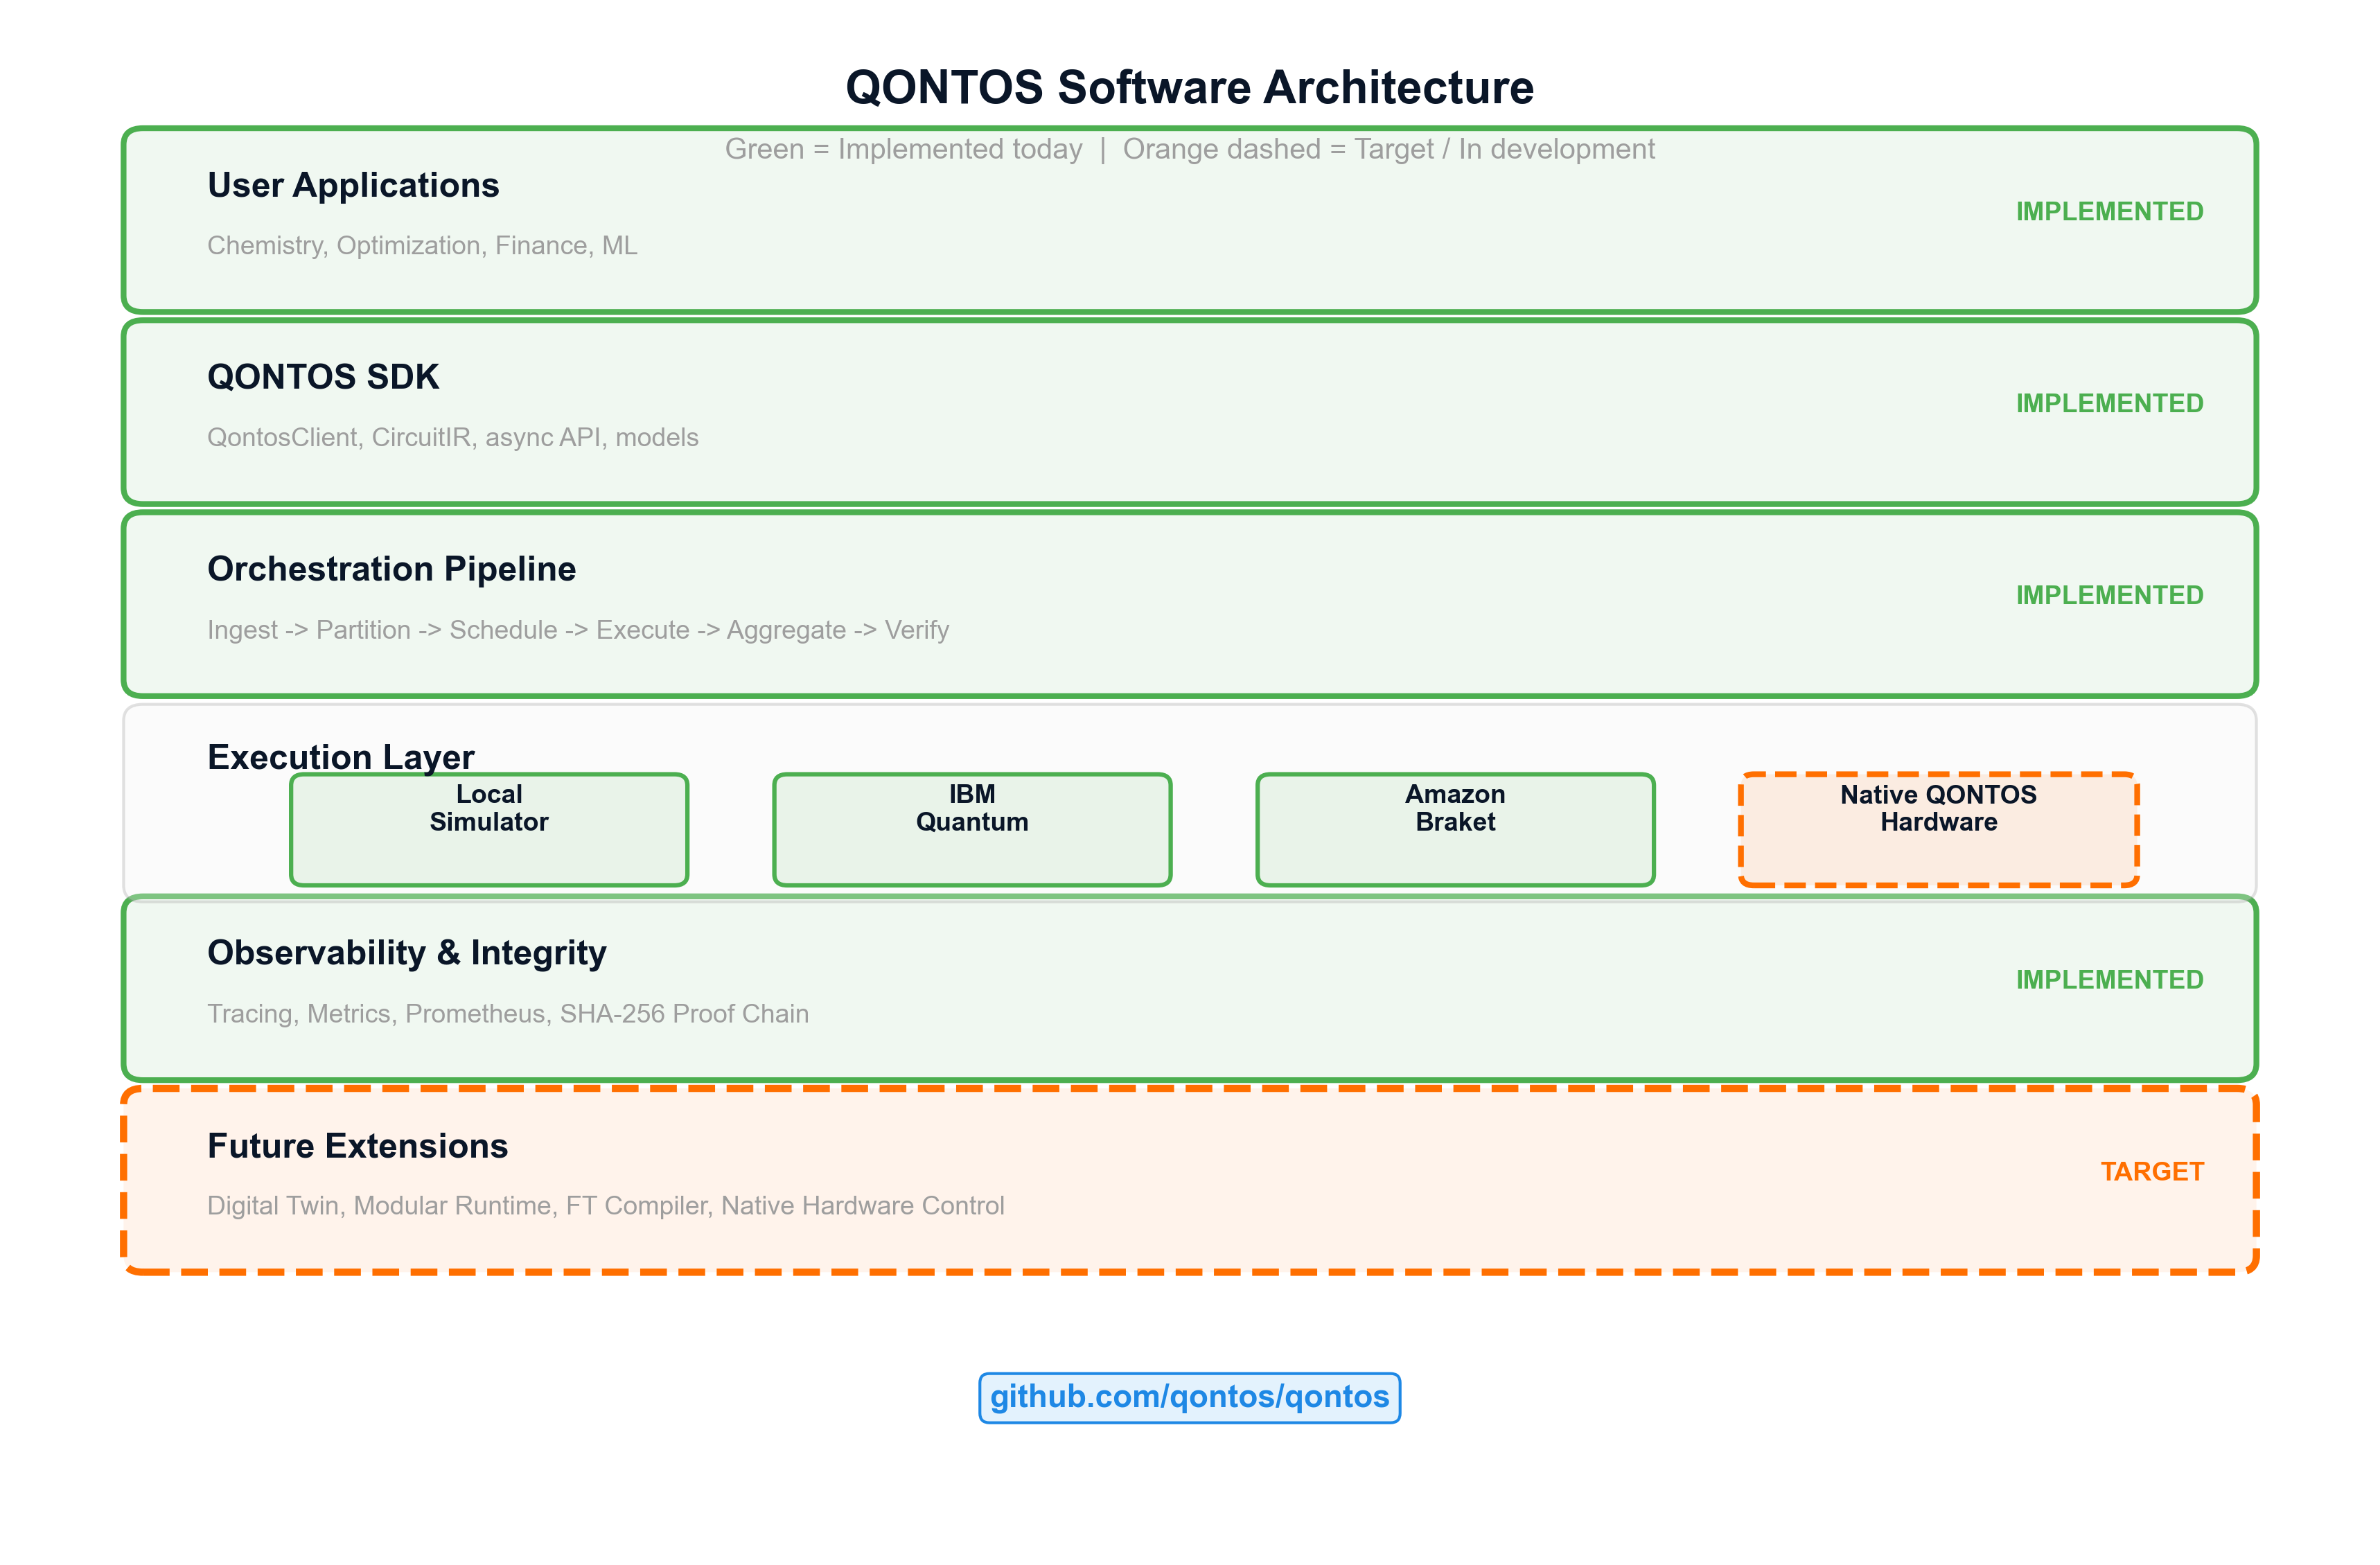
\includegraphics[width=\columnwidth]{../../figures/06_software_stack.png}
\caption{QONTOS software architecture overview.}
\label{fig:software-arch}
\end{figure}

\textbf{[Claim: IMPLEMENTED---all components in this section run today on simulator backends]}

The QONTOS platform implements a six-stage orchestration pipeline that orchestrates circuits across photonically-interconnected superconducting modules. Each stage corresponds to a module in the codebase. The software stack is designed from the ground up for the hybrid superconducting-photonic modular architecture, where superconducting processor modules are linked via photonic interconnects.

\subsection{Circuit Ingestion and Normalization}

The ingestion layer accepts quantum circuits in OpenQASM~3~\cite{Cross2022} and Qiskit circuit-object formats. Circuits are parsed, validated for gate-set compliance, and normalized into an internal directed-acyclic-graph (DAG) representation that preserves gate ordering, classical control dependencies, and measurement operations. Metadata---circuit name, qubit count, gate depth, submission timestamp---is attached at ingestion and propagated through the entire pipeline. The ingestion module handles circuits up to several hundred qubits on simulator backends with no hardware-specific transpilation.

\subsection{Circuit Partitioning}

The partitioning engine decomposes circuits into sub-circuits for independent execution. On simulator backends, partitioning enables parallel simulation and establishes the algorithmic foundation for future multi-module execution. The partitioner uses graph-bisection on the circuit DAG, minimizing inter-partition edges (corresponding to cross-module entanglement in the hardware case). Partition metadata---cut locations, estimated communication cost, sub-circuit qubit counts---is recorded for downstream use.

\subsection{Scheduling and Resource Allocation}

The scheduler assigns sub-circuits to execution backends based on resource availability, estimated execution time, and partition dependencies. The model is priority-queue-based with dependency-aware ordering. The scheduler interface is backend-agnostic: any execution target conforming to the QONTOS backend protocol can register. When hardware backends become available, they will use the same interface.

\subsection{Execution Dispatch}

The dispatch layer sends scheduled sub-circuits to assigned backends, monitors execution status, handles timeouts, and collects raw results. It includes retry logic for transient failures and a dead-letter mechanism for permanently failed jobs.

\subsection{Result Aggregation and Provenance}

\textbf{[Claim: IMPLEMENTED]} The aggregation engine reconstructs global measurement distributions from sub-circuit results via classical post-processing. Every aggregation step is logged with full provenance: contributing sub-circuits, executing backends, wall-clock timing, and post-processing applied. Results are stored in a structured format supporting replay and audit.

\subsection{Observability and Replayability}

The observability layer provides structured logging, metrics emission, and full execution replay. Every pipeline run produces an execution trace enabling debugging, benchmarking (see Paper~09), and reproducibility via re-execution from recorded traces.

\begin{table}[H]
\centering
\caption{Current QONTOS pipeline stages and implementation status.}
\label{tab:pipeline-stages}
\footnotesize
\begin{tabularx}{\columnwidth}{L{2.5cm}L{2.5cm}l}
\toprule
\textbf{Pipeline Stage} & \textbf{Module} & \textbf{Status} \\
\midrule
Circuit ingestion & \texttt{ingestion/} & Implemented \\
Partitioning & \texttt{partitioning/} & Implemented \\
Scheduling & \texttt{scheduler/} & Implemented \\
Execution dispatch & \texttt{dispatch/} & Implemented \\
Result aggregation & \texttt{aggregation/} & Implemented \\
Observability & \texttt{observability/} & Implemented \\
\bottomrule
\end{tabularx}
\end{table}

\section{Platform Validation and Proof-of-Execution}

\textbf{[Claim: IMPLEMENTED]}

\subsection{Validation Mechanisms}

The current platform is validated through unit and integration tests covering nominal operation, edge cases, and failure modes; a benchmark suite measuring pipeline throughput, per-stage latency, and result fidelity (detailed in Paper~09); and a replay mechanism that re-executes stored traces and compares outputs to the original run.

\subsection{Proof-of-Execution}

QONTOS implements a proof-of-execution framework providing cryptographic attestation of pipeline runs. Each execution produces a signed record containing: input circuit hash, partition plan hash, per-backend execution receipts, aggregated result hash, and full provenance chain. This supports use cases where computation results must be auditable.

\textbf{Current limitation:} Proof-of-execution currently attests to simulator-based runs. Hardware attestation introduces challenges (calibration state verification, hardware identity authentication) not yet addressed.

\section{Target Eight-Layer Architecture}

\textbf{[Claim: TARGET---this section describes architectural goals, not implemented capability]}

The full QONTOS software stack targets an eight-layer architecture spanning from physical hardware to end-user applications.

\begin{table}[H]
\centering
\caption{Eight-layer target architecture with implementation status.}
\label{tab:eight-layer}
\footnotesize
\begin{tabularx}{\columnwidth}{clL{2.5cm}l}
\toprule
\textbf{Layer} & \textbf{Name} & \textbf{Function} & \textbf{Status} \\
\midrule
8 & Applications & Domain-specific quantum apps & Target \\
7 & Algorithms & Algorithm libs \& hybrid workflows & Target \\
6 & Compilation & Circuit opt., partitioning, cutting & Partial \\
5 & Runtime & Execution orch., resource mgmt. & Partial \\
4 & ISA Abstr. & HW-agnostic instruction interface & Target \\
3 & Cross-Mod. & Inter-module timing, entangle.\ sched. & Target \\
2 & Control/Cal. & Real-time pulse ctrl, calib.\ feedback & Target \\
1 & HW/Photonics & Physical qubits, interconnects, cryo. & Target \\
\bottomrule
\end{tabularx}
\end{table}

The layered design follows the principle that quantum software stacks benefit from the same separation of concerns that made classical computing scalable~\cite{Heim2020}. Each layer exposes a well-defined interface to the layer above, hiding implementation details below. The implemented platform currently covers the core of Layers~5 and~6; the target extends downward toward hardware (Layers~1--4) and upward toward applications (Layers~7--8).

\subsection{ISA and Hardware Portability}

The target ISA layer (Layer~4) will accept optimized circuits in OpenQASM~3~\cite{Cross2022}, translate abstract gate operations into hardware-native sequences, and provide an abstraction boundary isolating upper layers from hardware specifics. This enables the same scheduling and partitioning logic to target different qubit technologies by swapping only the ISA implementation.

\section{Target Modular Runtime Extensions}

\textbf{[Claim: TARGET---none of the capabilities below are implemented today]}

\subsection{Module-Aware Circuit Placement}

The target placement engine will extend the current graph-bisection partitioner with topology constraints (mapping partitions to physical modules based on interconnect adjacency), calibration-aware scoring (weighting assignments by current gate fidelity and coherence time), and load balancing across modules. This is informed by modular architecture research~\cite{Monroe2014} and distributed quantum computing ecosystem literature~\cite{Cuomo2020}.

\subsection{Communication-Aware Scheduling}

Inter-module entanglement operations are orders of magnitude slower than local gates. The target scheduler will explicitly model communication cost, scheduling local operations in parallel with inter-module entanglement generation to maximize throughput.

\subsection{Dynamic Calibration Integration}

The target runtime will consume calibration telemetry from the control layer and adjust scheduling and placement decisions in near-real-time. If a module's fidelity drops below threshold, the scheduler will reroute workload to healthier modules.

\subsection{Fault-Tolerant Workload Control}

For error-corrected workloads, the target runtime will provide logical-qubit lifecycle management, syndrome extraction scheduling synchronized across modules, and decoder result integration for real-time error correction decisions (interfacing with Paper~05).

\section{Circuit Cutting and Distributed Reconstruction}

\textbf{[Claim: PARTIAL]}

\begin{itemize}
\item \textbf{Current capability (implemented):} The partitioning engine identifies cut points minimizing classical reconstruction overhead. Sub-circuits execute independently on simulator backends; results are reconstructed via the aggregation engine.
\item \textbf{Target extension:} Circuit cutting will integrate with the placement engine (Section~5.1) and communication-aware scheduler (Section~5.2), placing cuts to respect physical module boundaries and inter-module bandwidth constraints.
\end{itemize}

\section{Target Capability by Scale Phase}

\textbf{[Claim: TARGET---projected milestones, not commitments]}

\begin{table}[H]
\centering
\caption{Target software capability by hardware scale phase.}
\label{tab:scale-phases}
\footnotesize
\begin{tabularx}{\columnwidth}{lclL{2.5cm}}
\toprule
\textbf{Phase} & \textbf{Modules} & \textbf{Log.\ Qubits} & \textbf{Key SW Milestone} \\
\midrule
1: Foundation & 1 & 0 (physical) & Current platform validated \\
2: Single-Mod.\ HW & 1 & 1--4 & HW backend integration \\
3: Multi-Module & 2--8 & 4--50 & Cross-module sched., placement \\
4: System Scale & 8--64 & 50--1,000 & Full 8-layer stack operational \\
5: Datacenter & 64+ & 1,000+ & Distributed runtime, hier.\ sched. \\
\bottomrule
\end{tabularx}
\end{table}

\textbf{Phase 1 is current.} All subsequent phases depend on hardware availability and continued software development.

\subsection{AI-Powered Optimization Targets}

\begin{table}[H]
\centering
\caption{AI optimization targets (projections, not benchmarked results).}
\label{tab:ai-opt}
\footnotesize
\begin{tabularx}{\columnwidth}{L{2.5cm}L{1.5cm}L{1.5cm}L{1.5cm}}
\toprule
\textbf{Function} & \textbf{Conservative} & \textbf{Moderate} & \textbf{Stretch} \\
\midrule
Gate count reduction & 10--15\% & 20--30\% & 40--50\% \\
Topology-aware mapping & Functional & Optimized & Near-optimal \\
Predictive calibration & Offline & Near-real-time & Real-time \\
\bottomrule
\end{tabularx}
\end{table}

\textbf{[Claim: TARGET]} These targets are informed by the circuit optimization literature. They have not been benchmarked on the current platform.

\section{Validation Gate: Digital Twin and Multi-Module Simulation}

\textbf{[Claim: TARGET]}

Before any target capability is promoted to ``implemented,'' it must pass the QONTOS validation gate:

\subsection{Digital Twin}

A digital twin of the target multi-module system will simulate module-level noise models, inter-module entanglement with realistic latency, calibration drift, and network topology constraints. Software extensions must demonstrate correct behavior on the digital twin before claiming hardware readiness.

\subsection{Validation Protocol}

\begin{enumerate}
\item \textbf{Functional correctness} on the digital twin for a reference circuit set
\item \textbf{Performance baseline} meeting defined throughput and latency thresholds
\item \textbf{Fault injection} handling simulated module failures and link outages
\item \textbf{Regression check} ensuring modular extensions do not degrade baseline capability
\end{enumerate}

\subsection{Promotion Criteria}

A target capability becomes ``implemented'' only when: digital twin validation passes all protocol steps, the capability is merged into the main branch, integration tests are added, and the paper section is updated with benchmarked results replacing projections.

\section{Relation to Existing Quantum Software Ecosystem}

The QONTOS software stack is not a replacement for existing frameworks. Circuit-level frameworks (Qiskit, PennyLane, t$|$ket$\rangle$, Cirq) focus on circuit construction, single-device optimization, and transpilation. QONTOS focuses on what happens after circuit construction: orchestrated execution across backends with partitioning, scheduling, aggregation, provenance, and observability. This is analogous to the classical distinction between a compiler (circuit framework) and an operating system (QONTOS).

Heim et al.~\cite{Heim2020} survey quantum programming languages and runtime models, identifying the need for richer runtime environments as quantum systems scale. QONTOS aligns with this trajectory.

\section{Limitations and Honest Assessment}

\subsection{What QONTOS Is Today}

QONTOS is a software orchestration platform running on classical simulators with a complete pipeline from circuit ingestion to result aggregation. The orchestration patterns, scheduling algorithms, and provenance mechanisms are non-trivial and designed to transfer to hardware backends.

\subsection{What QONTOS Is Not Today}

QONTOS does not run on quantum hardware. It has not demonstrated multi-module execution on physical devices. The target architecture (Sections~4--8) is a design, not an implementation. Performance projections are targets, not benchmarked results.

\subsection{Key Risks}

\begin{itemize}
\item \textbf{Hardware-software co-design gap:} Abstractions may need revision when hardware arrives.
\item \textbf{Calibration complexity:} Real-time calibration integration is substantially harder on physical hardware than in simulation.
\item \textbf{Communication bottleneck:} Near-term inter-module entanglement rates may be too low to support the scheduling models in Section~5.2.
\end{itemize}

\section{Conclusion}

The QONTOS software stack exists today as a working orchestration platform for quantum circuit execution on simulator backends. It provides circuit ingestion, partitioning, scheduling, execution dispatch, result aggregation, and observability---all implemented, tested, and available in the public repository.

The target extension toward a modular operating layer for multi-module quantum hardware is an architectural design informed by the distributed quantum computing literature. It is not yet implemented.

This honest separation---between what runs today and what we intend to build---is the most important feature of this paper. The quantum computing field benefits from platforms that build real capability incrementally rather than claiming future results as present achievements.

\begin{thebibliography}{8}

\bibitem{Cross2022}
A.~W.~Cross, L.~S.~Bishop, J.~A.~Smolin, and J.~M.~Gambetta, ``OpenQASM~3: A broader and deeper quantum assembly language,'' \emph{ACM Transactions on Quantum Computing}, vol.~3, no.~3, pp.~1--50, 2022.

\bibitem{Bergholm2022}
V.~Bergholm, J.~Izaac, M.~Schuld, C.~Gogolin \emph{et~al.}, ``PennyLane: Automatic differentiation of hybrid quantum-classical computations,'' arXiv:1811.04968, 2022.

\bibitem{Qiskit2023}
Qiskit contributors, ``Qiskit: An open-source framework for quantum computing,'' Zenodo, 2023. \url{https://doi.org/10.5281/zenodo.2573505}

\bibitem{LaRose2019}
R.~LaRose, A.~Tikku, E.~O'Neel-Judy, L.~Cincio, and P.~J.~Coles, ``Overview and comparison of gate level quantum software platforms,'' \emph{Quantum}, vol.~3, p.~130, 2019.

\bibitem{Heim2020}
B.~Heim, M.~Soeken, S.~Marshall, C.~Granade, M.~Roetteler, A.~Geller, M.~Troyer, and K.~Svore, ``Quantum programming languages,'' \emph{Nature Reviews Physics}, vol.~2, pp.~709--722, 2020.

\bibitem{Sivarajah2020}
S.~Sivarajah, S.~Dilkes, A.~Cowtan, W.~Simmons, A.~Edgington, and R.~Duncan, ``t$|$ket$\rangle$: A retargetable compiler for NISQ devices,'' \emph{Quantum Science and Technology}, vol.~6, no.~1, p.~014003, 2020.

\bibitem{Monroe2014}
C.~Monroe, R.~Raussendorf, A.~Ruthven, K.~R.~Brown, P.~Maunz, L.-M.~Duan, and J.~Kim, ``Large-scale modular quantum-computer architecture with atomic memory and photonic interconnects,'' \emph{Physical Review A}, vol.~89, no.~2, p.~022317, 2014.

\bibitem{Cuomo2020}
D.~Cuomo, M.~Caleffi, and A.~S.~Cacciapuoti, ``Towards a distributed quantum computing ecosystem,'' \emph{IET Quantum Communication}, vol.~1, no.~1, pp.~3--8, 2020.

\end{thebibliography}

\end{document}
